\documentclass{article}

\usepackage[utf8]{inputenc}
\usepackage[T1]{fontenc}
\usepackage[francais]{babel}
\usepackage{titling}
\setlength{\droptitle}{-3cm}
\usepackage{graphicx}
\usepackage{underscore}
\usepackage{hyperref} 


\title{Compte rendu : Jour 2}
\author{CAROT Axel, ARISOY Ivan Can, \\ BREILLAD Matis, BELKHITER Medhi}
\date{\today}

\begin{document}
\maketitle

\section{Travail effectué}

\subsection{Graphique en bulle}

\begin{figure}[h]
    \centering
    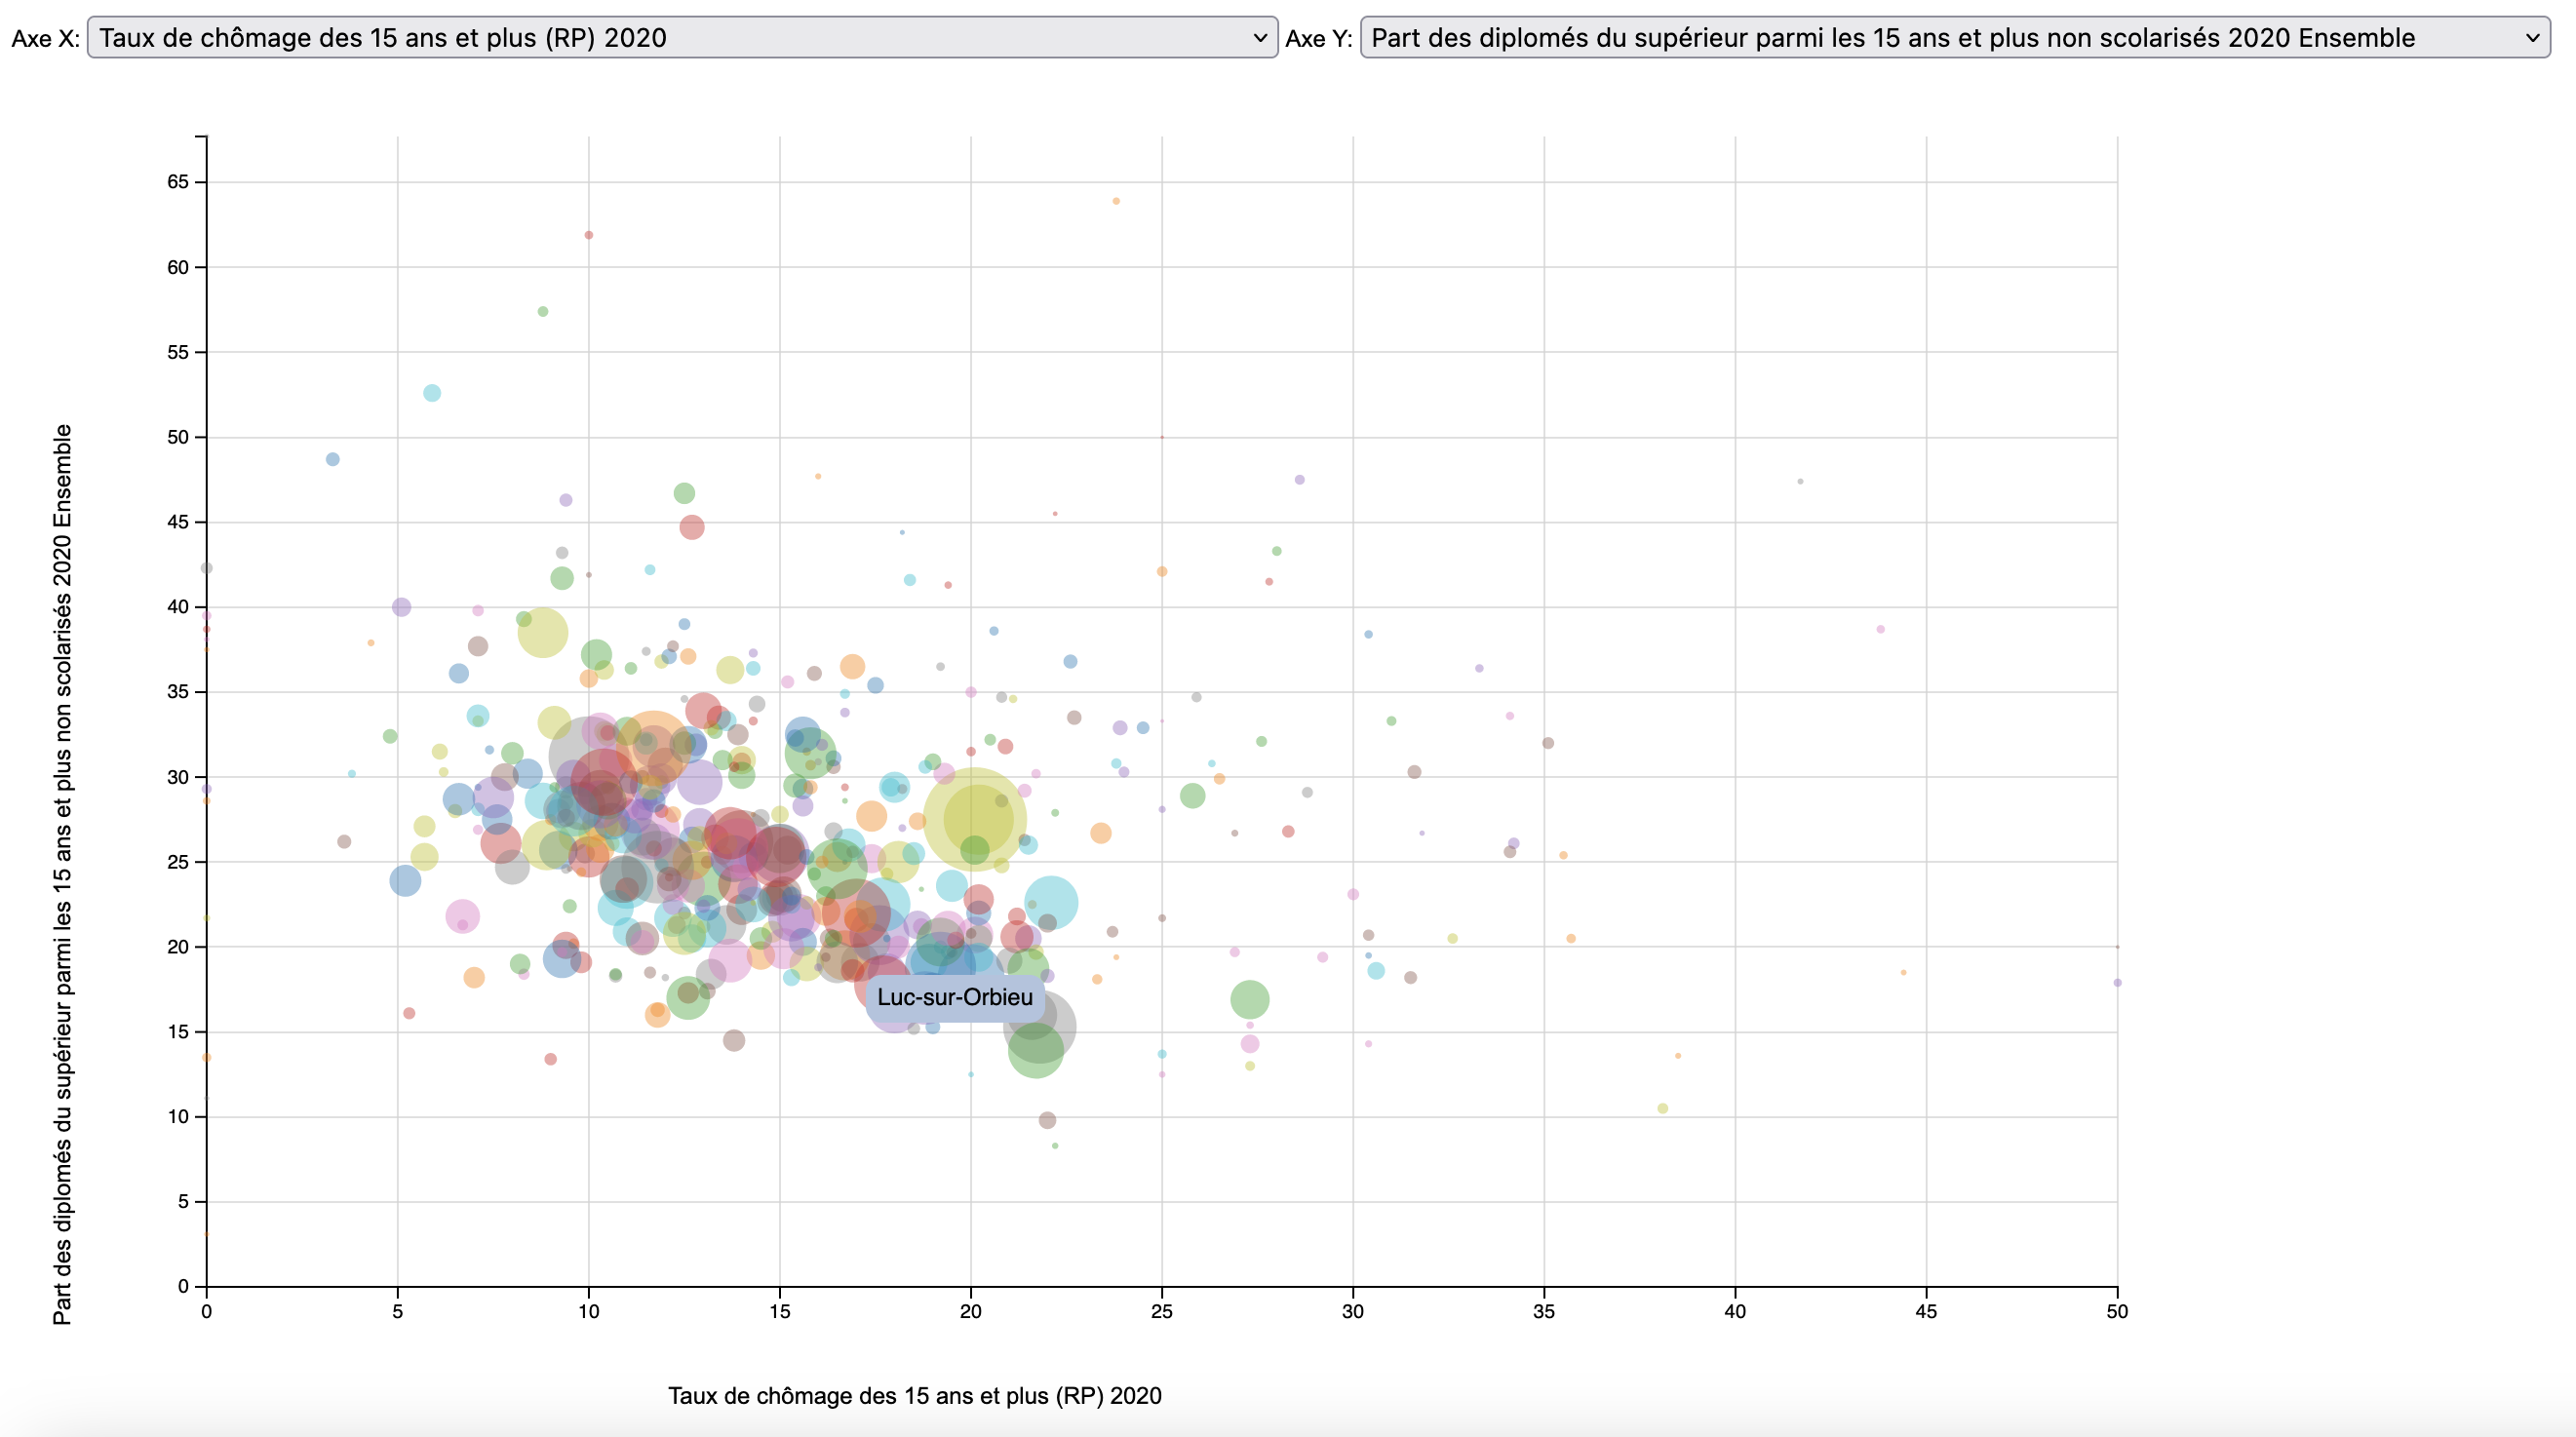
\includegraphics[width=1\textwidth]{bulle.png}
    \caption{Graphique en bulle}
    \label{fig:kaggle}
\end{figure}

Aujourd'hui, nous avons poursuivi notre travail en intégrant la fonctionnalité de zoom à notre graphique pour permettre une exploration plus détaillée des données. Nous avons également optimisé la taille des cercles pour les rendre proportionnels à la densité de population de chaque commune. Nous avons ajouté des couleurs distinctes pour chaque commune, ce qui permet de mieux distinguer les données sur la carte. Le graphique offre également une identification instantanée des communes grâce à l'affichage du nom lors du survol des cercles. \\

Cette visualisation interactive offre une grande flexibilité aux décideurs en leur permettant de comparer n'importe quelle variable en tant qu'axe X et Y. Cette fonctionnalité leur permet d'explorer les données selon leurs besoins spécifiques.
\vspace{2cm}
\subsection{Carte}

\begin{figure}[h]
    \centering
    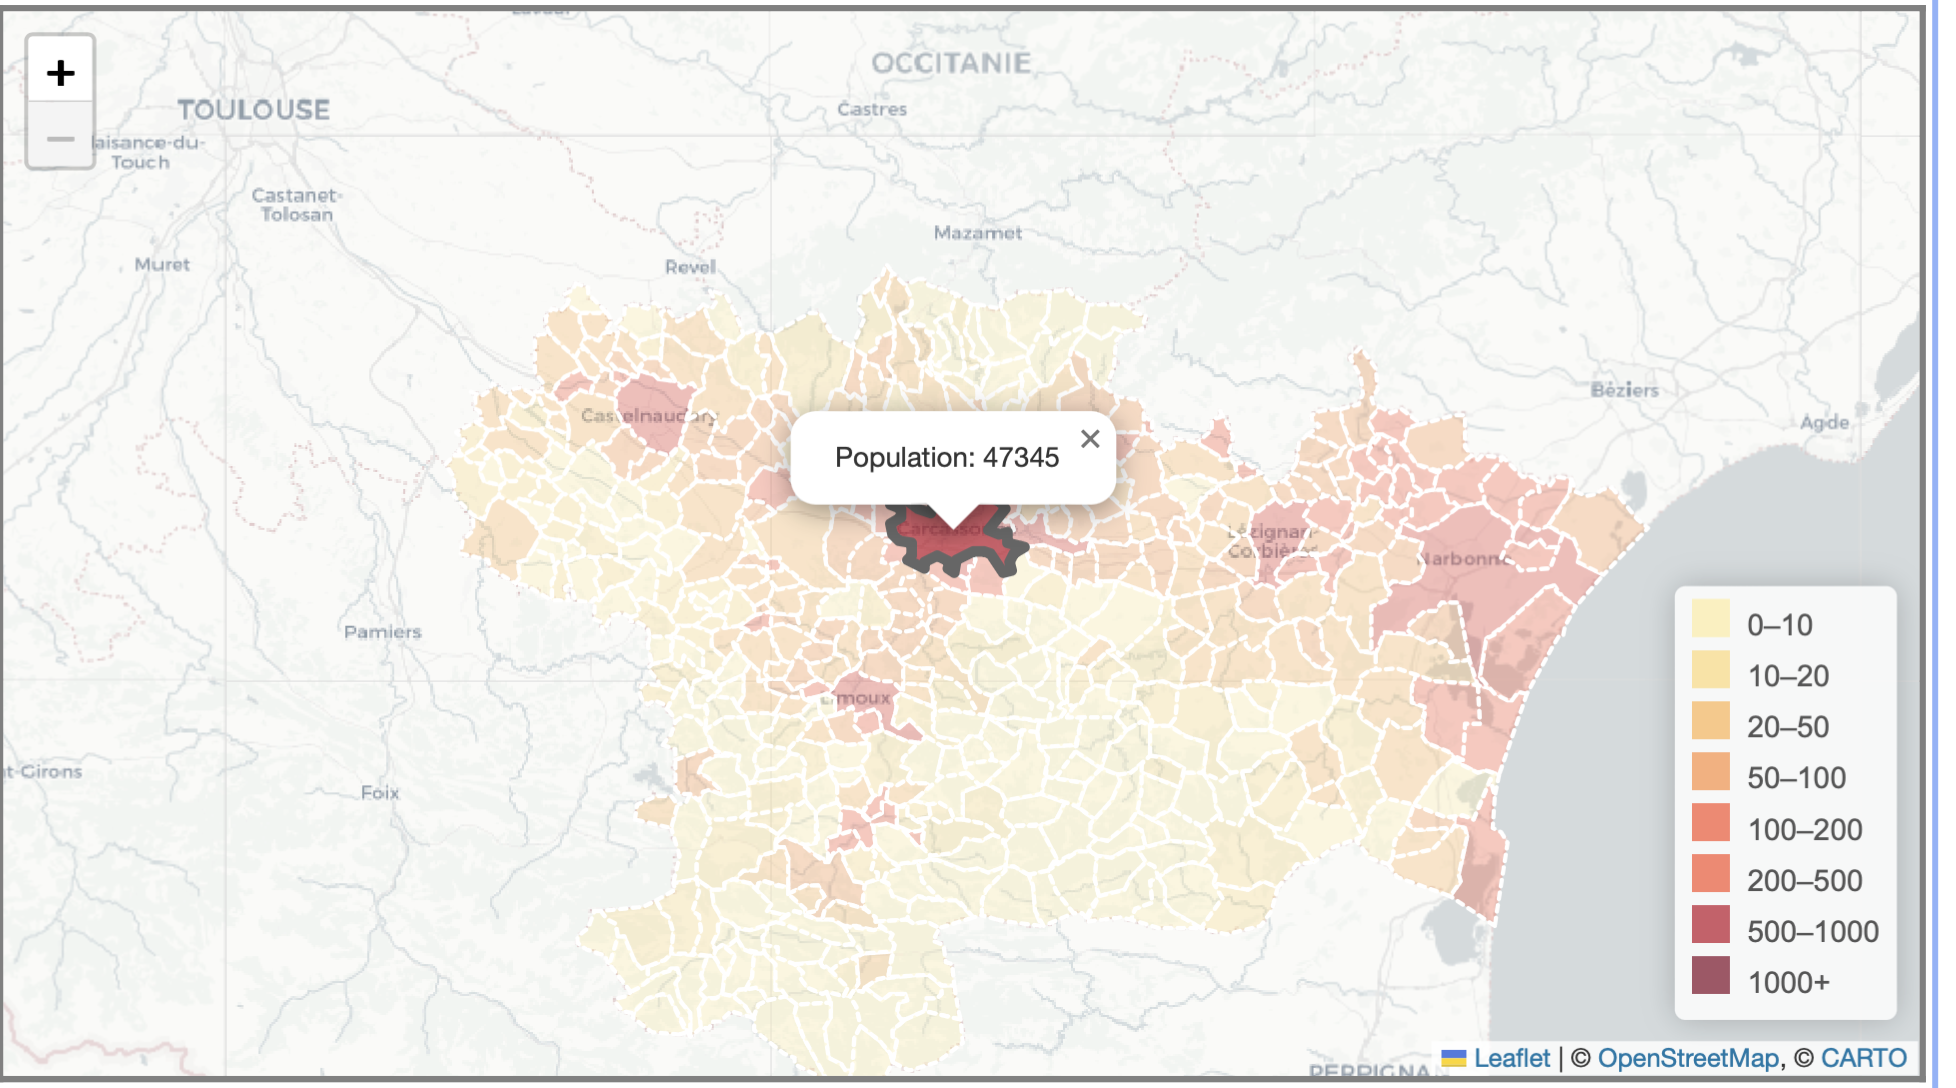
\includegraphics[width=1\textwidth]{carte.png}
    \caption{Graphique en bulle}
    \label{fig:kaggle}
\end{figure}

Nous avons lancé notre projet d'initialisation de carte interactive de la région en utilisant Leaflet et D3. En survolant les communes, les utilisateurs peuvent visualiser instantanément la population respective grâce à une superposition de données. De plus, nous avons ajouté une dimension visuelle en attribuant des codes couleur aux différentes zones en fonction de leur densité de population (qui sera remplacé par le score de l'indicateur que nous développerons).

\subsection{Site}

\begin{figure}[h]
    \centering
    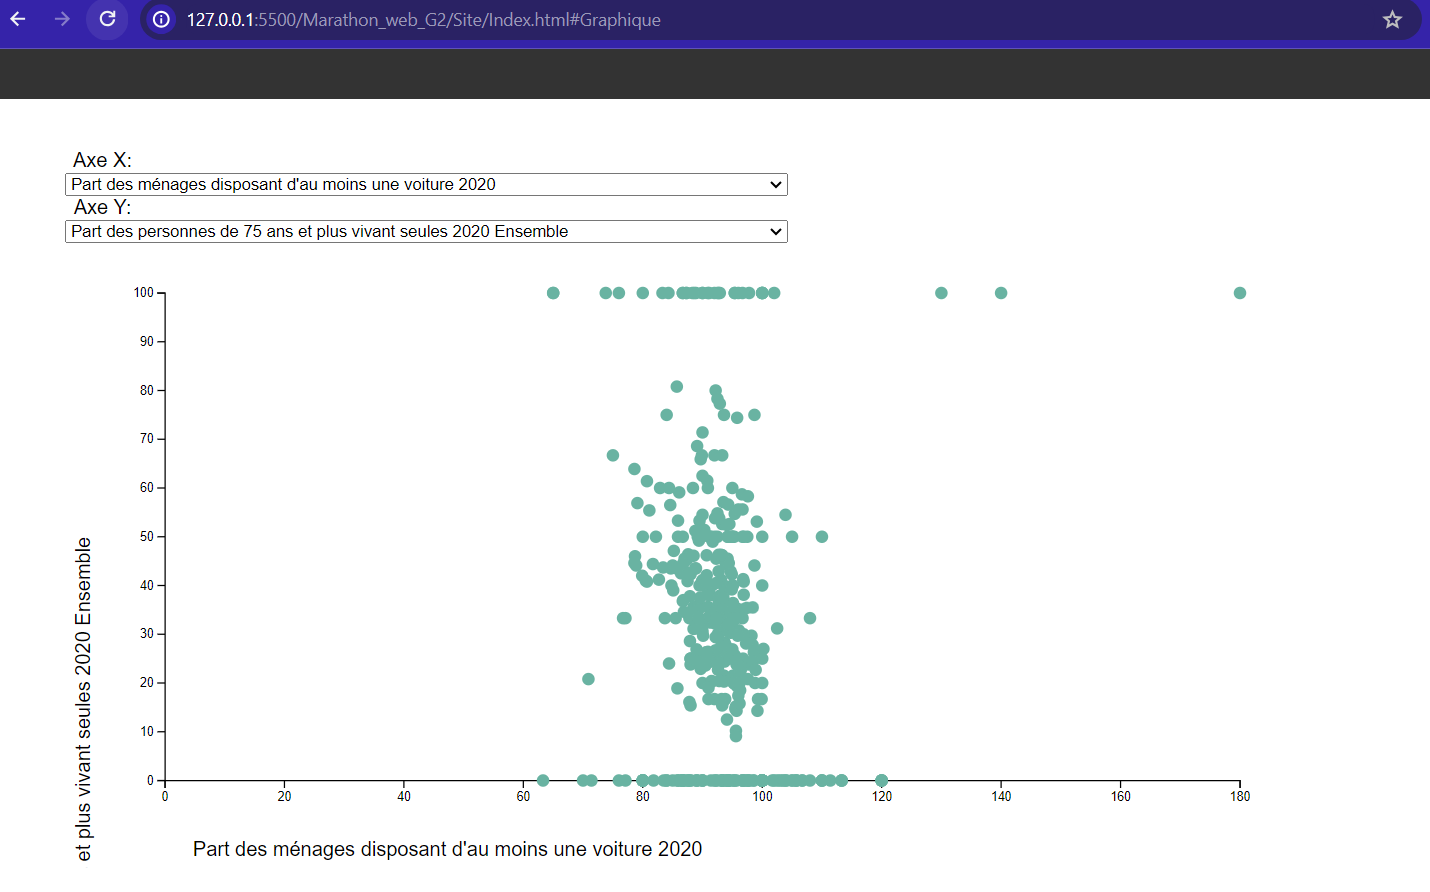
\includegraphics[width=0.7\textwidth]{site.png}
    \caption{Graphique en bulle}
    \label{fig:kaggle}
\end{figure}

Nous avons commencé à intégrer sur un site local nos outils de visualisations de données. Le screen montre le début de nos avancé pour intégrer le graphique en bulle.

\section{Travail à faire}
\begin{itemize}
    \item Finaliser le radar plot avec D3.
    \item Développer l'indicateur.
    \item Réaliser un mode d'emploie de l'outil de Data viz.
    \item Continuer nos avancé sur le site qui regroupe les outils de visualisation.
\end{itemize} 

\section{Problèmes rencontrés}
Nous avons des problèmes liés à l'affichage du radar plot avec D3. Nous avons aussi des difficultés pour assembler les différentes visualisations sur un même site et les reliés à un choix de variables.

\end{document}
